\documentclass[12pt]{article}
\usepackage{amsmath}
\usepackage[utf8]{inputenc}
\usepackage{float}
\usepackage{graphicx}
\usepackage[T1]{fontenc}

\DeclareGraphicsExtensions{.png}
%grafici
\usepackage{pgfplots}
\usetikzlibrary{patterns}
\pgfplotsset{/pgf/number format/use comma,compat=newest}

\usepackage{listings}
\renewcommand{\lstlistingname}{Codice}

\lstset{
  basicstyle=\footnotesize,
  numberstyle=\footnotesize,
  stepnumber=2,
  numbersep=5pt,
  backgroundcolor=\color{white},
  showspaces=false,
  showstringspaces=false,
  showtabs=false,
  frame=single,
  tabsize=4,
  captionpos=b,
  breaklines=true,
  breakatwhitespace=false,
  escapeinside={\%*}{*)},
  mathescape=true,
  morekeywords={
    begin,
    end,
    if,
    then,
    else,
    to,
    in,
    and,
    select,
    endif,
    Procedure,
    while,
    do,
    return,
    true,
    false,
    set,
    for,
    repeat,
    until,
    foreach,
    sort,
    count},
}


\begin{document}
\section*{Report: Collaborative Filtering}
\title{Collaborative Filtering Recommender Systems}

\paragraph*{Docente: }
Prof.essa Valentina Poggioni

\paragraph*{Studente: }
Matteo Capparrucci (280278)


\subsection*{Introduzione}
L'obiettivo di questa tesina è quello di fornire una panoramica generale nell'ambito dei Recommender System e, nello specifico, di quelli basati sulla tecnica del collaborative filtering basato sul calcolo delle misure di similarità User-User e Item-Item. Il dataset su cui sono stati svolti tutti i test è quello di MovieLens (sezione \ref{sec:MovieLens}), mentre i Raccommender System utilizzati per i vari casi di studio sono dei semplici algoritmi di prova inventati da me.



\section{Il dataset: MovieLens}
\label{sec:MovieLens}

MovieLens\footnote{http://movielens.org/} è un sito nato con lo scopo di consigliare film agli utenti basandosi sullo storico delle preferenze degli stessi. Il gruppo di ricerca GroupLens ha ricavato dal sito una ricca serie di dataset\footnote{il dataset è reperibile al link http://grouplens.org/datasets/movielens/} che, come anticipato, sono stati da me utilizzati per eseguire i test sulle performance dei vari reccomender system.
I dati contenuti rappresentano la popolazione e le conseguenti votazioni del sito, dalla sua apertura fino a delle date specifiche.
Per la precisione quelli utilizzati in questo lavoro sono:
\begin{itemize}
\item{MoviLens100K:}  Stabile dataset di benchmark contenente $100,000$ ratings da $1000$ utenti (ognuno con almeno 20 differenti recensioni) su circa $1700$ film rilasciata nell'aprile 1998.
\item{MoviLens1M:} \label{MoviLens1M} Stabile dataset di benchmark contenente $1,000,000$ ratings da $6000$ utenti (ognuno con almeno 20 differenti recensioni) su circa $4000$ film rilasciata nel febbraio del 2003.
\end{itemize}

\subsection{MoviLens100K}
\label{MoviLens100K}
MoviLens100K è il più piccolo della famiglia di dataset MovieLens e conseguentemente il più maneggevole, per questo motivo è anche il dataset sul quale sono stati eseguiti il numero maggiore di test e il debug vero e proprio degli algoritmi.

Nella figura \ref{fig:1}, osserviamo sull'asse delle y il numero di recensioni per ogni item e sull'asse delle x il numero di item aventi quel numero (y) di recensioni, una parte significativa degli oggetti recensiti nel dataset risultano avere un numero molto basso di recensioni.
Nell'ottica di alleggerire il carico computazionale necessario per il calcolo delle misure di similarità e rendere queste più efficaci, eseguiremo dei test eliminando gli oggetti con numero di recensioni totali minore di 5.

%Asse y: num di valutazioni Asse x: item ordinati secondo il num. di valutazioni in modo da trovare un ounto sull'asse y che permette di filtrare (ma non troppo)  gli item con poche valutazioni.

\begin{figure}[H]
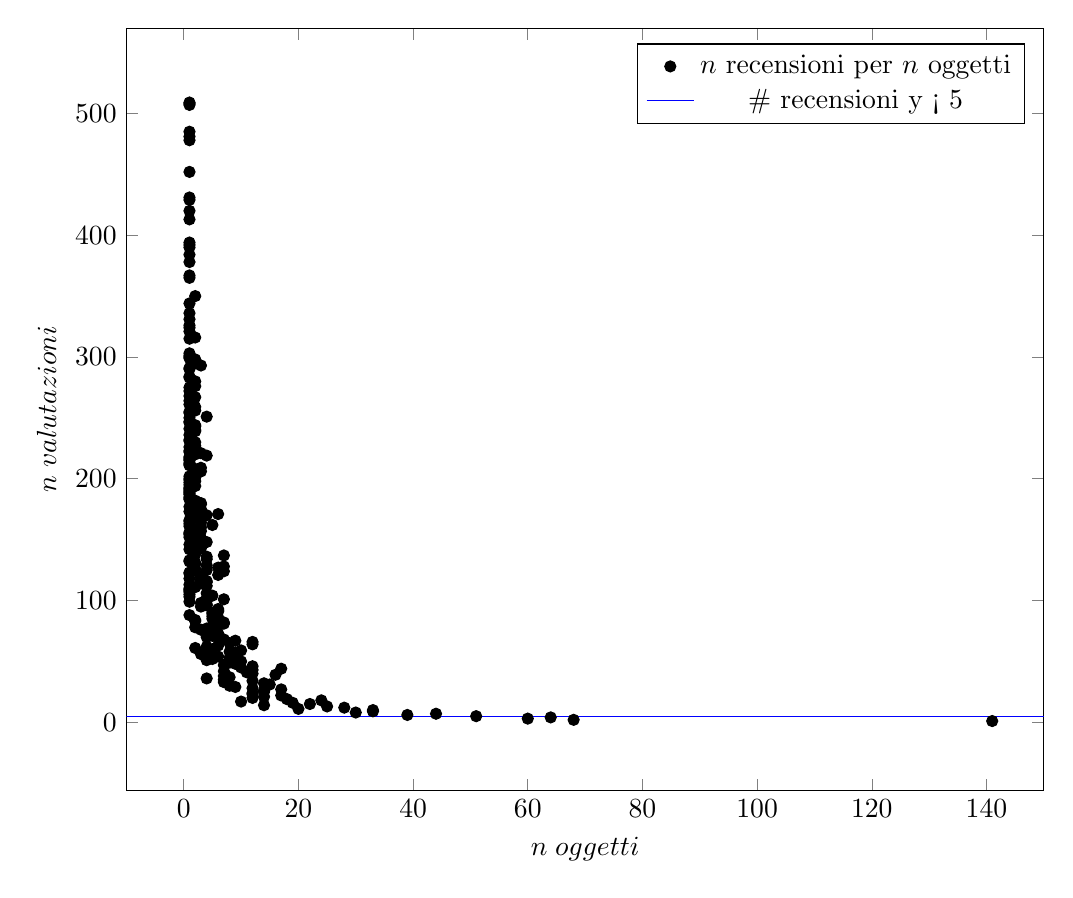
\begin{tikzpicture}
\begin{axis}[scale=1.7,xlabel=$n \; oggetti$,ylabel=$n \; valutazioni$, legend style={at={(0.98,0.98)},anchor=north east},ymax=570,xmax=150,xmin=-10]
\addplot[
%        thick,
		only marks,
        mark=*,
        black
      ] plot coordinates
{
 (141, 1) (68, 2) (60, 3) (64, 4) (51, 5) (39, 6) (44, 7) (30, 8) (33, 9) (33, 10) (20, 11) (28, 12) (25, 13) (14, 14) (22, 15) (19, 16) (10, 17) (24, 18) (18, 19) (12, 20) (14, 21) (17, 22) (12, 23) (12, 24) (14, 25) (14, 26) (17, 27) (12, 28) (9, 29) (8, 30) (15, 31) (14, 32) (7, 33) (12, 34) (7, 35) (4, 36) (8, 37) (7, 38) (16, 39) (12, 40) (11, 41) (7, 42) (12, 43) (17, 44) (10, 45) (12, 46) (7, 47) (9, 48) (8, 49) (10, 50) (4, 51) (5, 52) (8, 53) (6, 54) (4, 55) (3, 56) (9, 57) (8, 58) (10, 59) (5, 60) (2, 61) (4, 62) (6, 63) (12, 64) (8, 65) (12, 66) (9, 67) (7, 68) (6, 69) (4, 70) (5, 71) (6, 72) (6, 73) (4, 74) (4, 75) (3, 76) (4, 77) (2, 78) (5, 79) (6, 80) (7, 81) (7, 82) (2, 83) (2, 84) (5, 85) (6, 86) (5, 87) (1, 88) (5, 89) (5, 90) (6, 91) (6, 92) (6, 93) (3, 95) (4, 96) (4, 97) (3, 98) (1, 99) (4, 100) (7, 101) (4, 102) (1, 103) (5, 104) (1, 105) (4, 106) (1, 107) (1, 108) (1, 109) (1, 110) (2, 111) (4, 112) (1, 113) (3, 114) (4, 115) (4, 116) (3, 117) (1, 118) (3, 119) (3, 120) (6, 121) (1, 122) (1, 123) (7, 124) (4, 125) (2, 126) (6, 127) (7, 128) (4, 129) (2, 130) (2, 131) (1, 132) (1, 133) (4, 134) (4, 136) (7, 137) (2, 138) (1, 142) (3, 143) (2, 145) (1, 146) (2, 147) (4, 148) (3, 149) (2, 150) (3, 151) (1, 152) (2, 153) (1, 154) (1, 155) (1, 156) (3, 157) (2, 158) (3, 160) (1, 161) (5, 162) (1, 163) (3, 164) (1, 165) (1, 166) (2, 168) (3, 169) (4, 170) (6, 171) (2, 172) (1, 173) (3, 174) (3, 175) (2, 176) (1, 177) (2, 178) (3, 179) (3, 180) (2, 182) (1, 183) (1, 184) (1, 185) (1, 187) (1, 188) (1, 189) (1, 190) (1, 191) (1, 192) (1, 193) (2, 194) (1, 195) (1, 197) (2, 198) (1, 199) (1, 200) (2, 201) (1, 202) (3, 206) (2, 208) (3, 209) (1, 211) (1, 212) (1, 213) (1, 215) (1, 216) (1, 217) (1, 218) (4, 219) (2, 220) (3, 221) (1, 222) (1, 223) (1, 226) (2, 227) (2, 230) (1, 231) (1, 232) (1, 236) (2, 239) (2, 240) (1, 241) (2, 243) (2, 244) (1, 246) (1, 247) (1, 250) (4, 251) (1, 254) (1, 255) (2, 256) (2, 259) (1, 261) (1, 264) (2, 267) (1, 268) (1, 272) (1, 275) (2, 276) (2, 280) (1, 283) (1, 284) (1, 290) (1, 291) (3, 293) (2, 295) (2, 297) (2, 298) (1, 299) (1, 300) (1, 301) (1, 303) (1, 315) (2, 316) (1, 321) (1, 324) (1, 326) (1, 331) (1, 336) (1, 344) (2, 350) (1, 365) (1, 367) (1, 378) (1, 384) (1, 390) (1, 392) (1, 394) (1, 413) (1, 420) (1, 429) (1, 431) (1, 452) (1, 478) (1, 481) (1, 485) (1, 507) (1, 508) (1, 509) (1, 583) 


};


\addplot[mark=none, blue] coordinates {(-10,5) (500,5)};


\legend{$n$ recensioni per $n$ oggetti, \# recensioni y < 5}

\end{axis}
\end{tikzpicture}
\label{fig:1}
\caption{n oggetti x numero recensioni}
\end{figure}



\subsection{MoviLens1M}
\label{MoviLens1M}

MoviLens1M è un dataset di dimensione molto maggiore rispetto al precedente e dunque è stato utilizzato solo per pochi test dimostrativi vista la difficoltà (perlopiù temporale) data dal maneggiare un volume di dati di tali dimensioni.

Con il crescere del numero di review è possibile notare, come evidenziato in figura \ref{fig:2}, un'inversione di tendenza rispetto al dataset di 'taglia' minore, in questo caso infatti il rapporto tra utenti e oggetti è sbilanciato dalla parte dei primi, che sono oltre $6000$, in ogni caso, come con i precedenti è stato possibile eliminare una parte degli oggetti, eliminando quelli con numero di recensioni minori di 5, al fine di diminuire le dimensioni del dataset, e quindi consentire un calcolo più agevole della matrice di similarità e eliminare da essa i risultati meno significativi.


\begin{figure}[H]
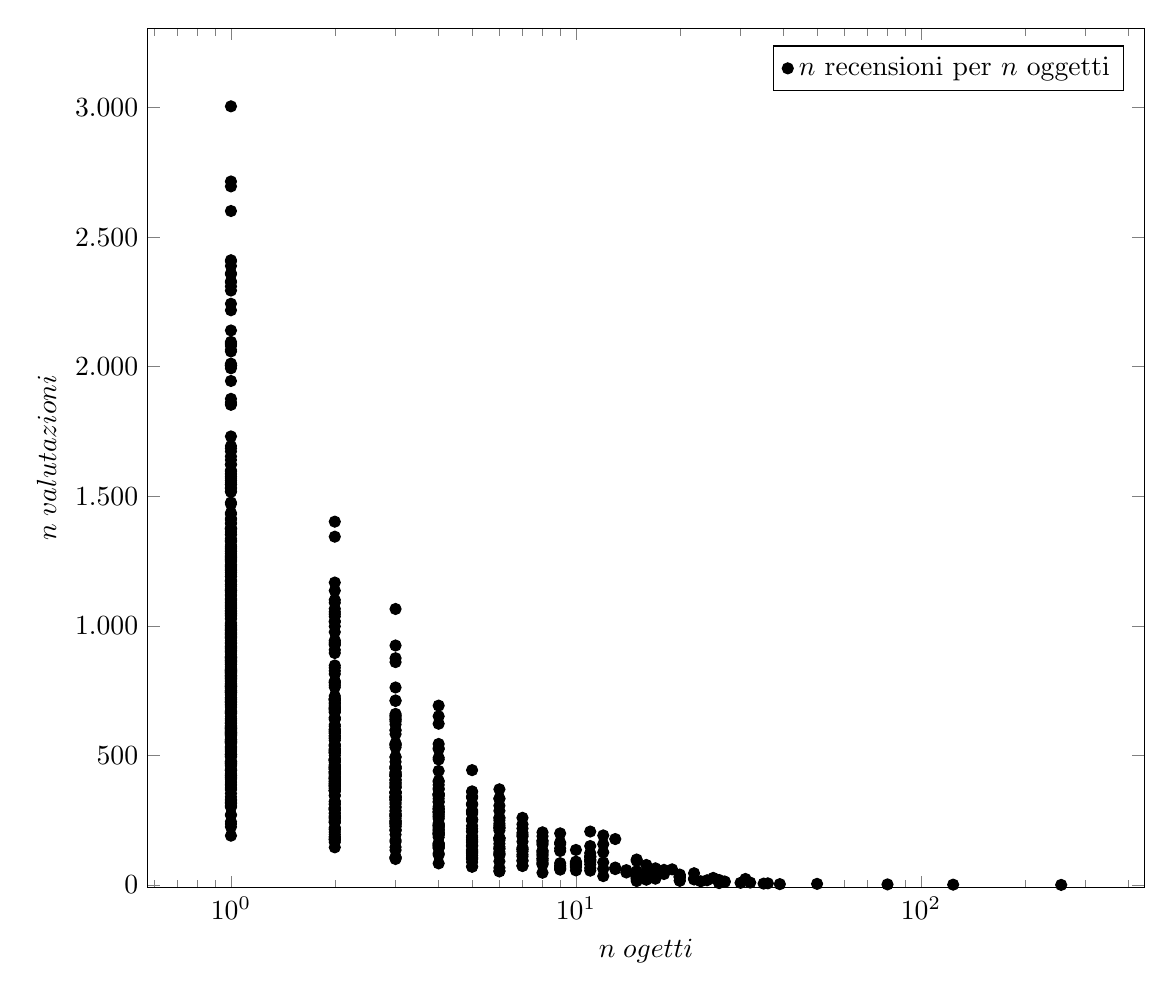
\begin{tikzpicture}
\begin{axis}[scale=1.5,xlabel=$n \; ogetti$,ylabel=$n \; valutazioni$,
xmode=log,
scale only axis,
log origin=infty,
legend style={at={(0.98,0.98)},anchor=north east},%ymax=300,
%xmax=800,
xmin=-10,ymin = -10]
\addplot[
%        thick,
		only marks,
        mark=*,
        black
      ] plot coordinates
{
(255,0) (124,1) (80,2) (50,4) (39,3) (36,6) (35,5) (32,9) (31,23) (30,8) (27,13) (27,12) (26,19) (26,11) (26,10) (26,7) (25,27) (24,18) (23,14) (22,45) (22,25) (22,21) (20,40) (20,35) (20,33) (20,32) (20,29) (20,28) (20,17) (20,16) (19,60) (18,58) (18,49) (18,42) (17,64) (17,39) (17,36) (17,24) (16,77) (16,51) (16,50) (16,43) (16,38) (16,37) (16,31) (16,20) (15,98) (15,93) (15,53) (15,46) (15,44) (15,41) (15,30) (15,26) (15,22) (15,15) (14,57) (14,48) (13,177) (13,67) (13,61) (12,191) (12,157) (12,126) (12,87) (12,62) (12,34) (11,206) (11,150) (11,123) (11,111) (11,109) (11,107) (11,97) (11,96) (11,89) (11,79) (11,65) (11,55) (10,135) (10,90) (10,85) (10,81) (10,80) (10,76) (10,72) (10,68) (10,56) (9,199) (9,164) (9,158) (9,141) (9,131) (9,84) (9,75) (9,69) (9,63) (9,59) (8,203) (8,188) (8,171) (8,169) (8,162) (8,155) (8,133) (8,130) (8,124) (8,118) (8,112) (8,102) (8,101) (8,94) (8,86) (8,82) (8,78) (8,47) (7,259) (7,234) (7,218) (7,201) (7,193) (7,187) (7,167) (7,144) (7,138) (7,137) (7,129) (7,117) (7,110) (7,95) (7,92) (7,74) (7,73) (6,369) (6,334) (6,332) (6,306) (6,286) (6,260) (6,258) (6,249) (6,237) (6,230) (6,223) (6,220) (6,219) (6,210) (6,182) (6,181) (6,180) (6,179) (6,172) (6,159) (6,147) (6,140) (6,139) (6,127) (6,120) (6,119) (6,114) (6,91) (6,66) (6,54) (6,52) (5,443) (5,361) (5,359) (5,342) (5,336) (5,314) (5,311) (5,309) (5,288) (5,283) (5,280) (5,274) (5,254) (5,253) (5,252) (5,251) (5,247) (5,228) (5,217) (5,207) (5,205) (5,189) (5,183) (5,176) (5,170) (5,168) (5,163) (5,153) (5,152) (5,149) (5,136) (5,132) (5,128) (5,125) (5,121) (5,115) (5,113) (5,106) (5,103) (5,99) (5,88) (5,71) (5,70) (4,692) (4,651) (4,622) (4,544) (4,528) (4,524) (4,491) (4,484) (4,440) (4,402) (4,398) (4,386) (4,373) (4,368) (4,352) (4,351) (4,349) (4,348) (4,347) (4,343) (4,333) (4,322) (4,319) (4,303) (4,296) (4,293) (4,292) (4,284) (4,282) (4,281) (4,279) (4,272) (4,266) (4,262) (4,255) (4,238) (4,232) (4,231) (4,229) (4,226) (4,221) (4,215) (4,212) (4,208) (4,202) (4,200) (4,198) (4,197) (4,196) (4,192) (4,184) (4,161) (4,160) (4,156) (4,154) (4,151) (4,148) (4,143) (4,142) (4,122) (4,116) (4,83) (3,1065) (3,924) (3,875) (3,860) (3,762) (3,712) (3,710) (3,660) (3,654) (3,652) (3,645) (3,639) (3,637) (3,630) (3,619) (3,598) (3,596) (3,582) (3,547) (3,543) (3,541) (3,539) (3,531) (3,495) (3,492) (3,475) (3,457) (3,456) (3,452) (3,450) (3,448) (3,436) (3,433) (3,428) (3,426) (3,425) (3,421) (3,420) (3,419) (3,407) (3,405) (3,404) (3,396) (3,393) (3,388) (3,382) (3,378) (3,376) (3,375) (3,360) (3,358) (3,357) (3,356) (3,355) (3,354) (3,345) (3,341) (3,339) (3,338) (3,337) (3,335) (3,329) (3,328) (3,327) (3,318) (3,312) (3,302) (3,298) (3,287) (3,285) (3,276) (3,273) (3,270) (3,268) (3,265) (3,264) (3,256) (3,248) (3,246) (3,245) (3,240) (3,239) (3,236) (3,233) (3,227) (3,225) (3,214) (3,211) (3,209) (3,194) (3,173) (3,166) (3,146) (3,134) (3,108) (3,105) (3,104) (3,100) (2,1402) (2,1344) (2,1167) (2,1136) (2,1100) (2,1089) (2,1066) (2,1054) (2,1045) (2,1036) (2,1018) (2,1015) (2,998) (2,976) (2,944) (2,937) (2,930) (2,926) (2,907) (2,895) (2,847) (2,838) (2,826) (2,814) (2,787) (2,782) (2,780) (2,771) (2,763) (2,729) (2,720) (2,718) (2,717) (2,715) (2,714) (2,711) (2,704) (2,700) (2,694) (2,687) (2,683) (2,682) (2,681) (2,676) (2,675) (2,668) (2,666) (2,646) (2,644) (2,638) (2,618) (2,612) (2,601) (2,599) (2,594) (2,592) (2,587) (2,585) (2,576) (2,574) (2,567) (2,565) (2,558) (2,542) (2,540) (2,538) (2,535) (2,526) (2,522) (2,520) (2,519) (2,514) (2,513) (2,511) (2,510) (2,508) (2,499) (2,487) (2,486) (2,485) (2,483) (2,482) (2,481) (2,480) (2,479) (2,474) (2,464) (2,461) (2,458) (2,455) (2,454) (2,453) (2,451) (2,449) (2,446) (2,445) (2,438) (2,437) (2,435) (2,434) (2,430) (2,429) (2,424) (2,418) (2,416) (2,413) (2,412) (2,411) (2,409) (2,408) (2,401) (2,400) (2,399) (2,394) (2,392) (2,390) (2,387) (2,384) (2,383) (2,381) (2,380) (2,374) (2,372) (2,366) (2,365) (2,364) (2,363) (2,362) (2,346) (2,344) (2,323) (2,321) (2,313) (2,310) (2,299) (2,297) (2,295) (2,294) (2,291) (2,290) (2,289) (2,278) (2,275) (2,267) (2,263) (2,261) (2,257) (2,250) (2,243) (2,242) (2,241) (2,222) (2,216) (2,213) (2,204) (2,195) (2,186) (2,185) (2,178) (2,175) (2,174) (2,165) (2,145) (1,3005) (1,2715) (1,2696) (1,2601) (1,2411) (1,2407) (1,2389) (1,2361) (1,2357) (1,2330) (1,2326) (1,2310) (1,2294) (1,2243) (1,2218) (1,2140) (1,2096) (1,2091) (1,2087) (1,2080) (1,2065) (1,2059) (1,2012) (1,2007) (1,2005) (1,2004) (1,2003) (1,1994) (1,1945) (1,1876) (1,1863) (1,1856) (1,1853) (1,1731) (1,1694) (1,1685) (1,1673) (1,1654) (1,1640) (1,1623) (1,1622) (1,1601) (1,1596) (1,1588) (1,1583) (1,1576) (1,1570) (1,1562) (1,1560) (1,1552) (1,1546) (1,1545) (1,1533) (1,1532) (1,1530) (1,1519) (1,1517) (1,1476) (1,1470) (1,1436) (1,1431) (1,1415) (1,1409) (1,1397) (1,1394) (1,1378) (1,1376) (1,1375) (1,1372) (1,1362) (1,1353) (1,1351) (1,1336) (1,1335) (1,1329) (1,1327) (1,1324) (1,1312) (1,1306) (1,1301) (1,1297) (1,1292) (1,1287) (1,1286) (1,1279) (1,1277) (1,1270) (1,1269) (1,1265) (1,1262) (1,1261) (1,1256) (1,1254) (1,1251) (1,1247) (1,1236) (1,1234) (1,1231) (1,1229) (1,1224) (1,1220) (1,1216) (1,1214) (1,1207) (1,1205) (1,1197) (1,1191) (1,1190) (1,1177) (1,1175) (1,1173) (1,1172) (1,1170) (1,1160) (1,1158) (1,1152) (1,1143) (1,1139) (1,1138) (1,1137) (1,1135) (1,1130) (1,1121) (1,1118) (1,1115) (1,1105) (1,1102) (1,1097) (1,1092) (1,1090) (1,1085) (1,1081) (1,1077) (1,1073) (1,1069) (1,1067) (1,1060) (1,1059) (1,1055) (1,1053) (1,1047) (1,1046) (1,1042) (1,1040) (1,1035) (1,1028) (1,1026) (1,1012) (1,1009) (1,1004) (1,1001) (1,1000) (1,999) (1,993) (1,989) (1,986) (1,984) (1,983) (1,981) (1,980) (1,974) (1,972) (1,969) (1,967) (1,964) (1,959) (1,957) (1,956) (1,954) (1,953) (1,951) (1,943) (1,936) (1,933) (1,931) (1,925) (1,920) (1,919) (1,917) (1,913) (1,910) (1,904) (1,903) (1,901) (1,897) (1,890) (1,882) (1,880) (1,879) (1,878) (1,877) (1,874) (1,872) (1,871) (1,866) (1,865) (1,864) (1,863) (1,859) (1,856) (1,851) (1,850) (1,843) (1,840) (1,836) (1,833) (1,831) (1,829) (1,828) (1,827) (1,824) (1,823) (1,821) (1,820) (1,818) (1,817) (1,815) (1,813) (1,809) (1,808) (1,807) (1,806) (1,804) (1,800) (1,798) (1,796) (1,795) (1,792) (1,788) (1,786) (1,784) (1,778) (1,776) (1,773) (1,769) (1,768) (1,767) (1,766) (1,765) (1,764) (1,761) (1,760) (1,757) (1,756) (1,751) (1,750) (1,748) (1,745) (1,744) (1,743) (1,742) (1,737) (1,736) (1,732) (1,723) (1,722) (1,721) (1,716) (1,713) (1,708) (1,707) (1,706) (1,705) (1,703) (1,702) (1,696) (1,695) (1,690) (1,684) (1,674) (1,671) (1,669) (1,667) (1,664) (1,663) (1,662) (1,650) (1,642) (1,640) (1,634) (1,629) (1,626) (1,625) (1,624) (1,623) (1,615) (1,614) (1,611) (1,609) (1,608) (1,605) (1,604) (1,603) (1,602) (1,600) (1,597) (1,595) (1,593) (1,591) (1,590) (1,589) (1,588) (1,586) (1,584) (1,583) (1,581) (1,579) (1,577) (1,575) (1,571) (1,563) (1,562) (1,561) (1,559) (1,556) (1,555) (1,554) (1,552) (1,551) (1,550) (1,548) (1,546) (1,534) (1,532) (1,529) (1,525) (1,521) (1,517) (1,516) (1,509) (1,505) (1,504) (1,503) (1,502) (1,497) (1,496) (1,493) (1,478) (1,477) (1,476) (1,472) (1,470) (1,469) (1,466) (1,463) (1,460) (1,459) (1,447) (1,444) (1,442) (1,441) (1,431) (1,427) (1,423) (1,422) (1,417) (1,414) (1,410) (1,406) (1,397) (1,389) (1,385) (1,377) (1,371) (1,367) (1,353) (1,340) (1,330) (1,325) (1,320) (1,317) (1,316) (1,315) (1,305) (1,304) (1,300) (1,271) (1,269) (1,244) (1,235) (1,224) (1,190)

};


\legend{$n$ recensioni per $n$ oggetti}
\end{axis}
\end{tikzpicture}
\label{fig:2}
\caption{n oggetti x numero recensioni}
\end{figure}


\section{Recommender System}

Come anticipato, lo scopo di questi test era quello di valutare e testare alcuni semplici reccommender system, basati sulla tecnica del collaborative filtering, sui dataset MoviLens. 

Un recommender system è un particolare tipo di algoritmo finalizzato alla formulazione di un rating o di una preferenza per un dato utente su un dato item. Nel caso dei reccomender system basati sul collaborative filtering questa 'predizione' viene formulata a partire da un modello costruito sulla base di informazioni storiche degli utenti.

Entrambi gli algortimi proposti calcolano quindi per prima cosa  una 'misura di similarità', sugli utenti o sugli item, utilizzando i dati sul comportamento passato degli utenti. Nel caso di algoritmi più evoluti vengono inoltre estratte delle ulteriori feature, anche non banalmente correlate al dato da predire, per raffinare la qualità dell'output.

In questo caso, comunque, la matrice di similarità sarà calcolata utilizzando la misura di similarità secondo Pearson, che è una delle più comuni e note.

\subsection{Pearson Correlation Similarity}
\label{sec:Pearson Correlation Similarity}

La similarità secondo Pearson è una delle misure più utilizzate per la realizzazione di recommender system basati sul vicinato (Nearest Neighbor algorithm), che rientrano nella famiglia dei collaborative filtering user-based. Nello specifico, questa consente di rappresentare il grado di 'similarità' tra due utenti $x$ e $y$ (nel caso della user-user) sulla base dei voti che questi hanno dato a degli oggetti comuni $r_{x,i},r_{y,i}  : i \in I$ e alla media aritmetica dei loro voti totali $\overline{r}_{x}$ e $\overline{r}_{y}$ (tramite l'equazione \ref{Eq:1}).


\begin{equation}
simil(x,y) = \frac{\sum_{i \in I_{x,y}}(r_{x,i}-\overline{r}_{x})(r_{y,i}-\overline{r}_{y})}{\sqrt{\sum_{i \in I_{x,y}}(r_{x,i}-\overline{r}_{x})^2}\sqrt{\sum_{i \in I_{x,y}}(r_{y,i}-\overline{r}_{y})^2}}
\label{Eq:1}
\end{equation}

La stessa equazione, in ogni caso, può essere utilizzata anche per calcolare la similarità item-item selezionando opportunamente l'insieme dei vicini affinché rappresenti per ogni item $x$ il gruppo di utenti $I$ che hanno votato $x$.

Nel corso dei vari test, si è inoltre notato come l'equazione seguente fosse più efficiente rispetto alla precedente.

\begin{equation}
simil(x,y) = \frac{\sum_{i \in I_{x,y}}(r_{x,i}-\overline{r}_{x})(r_{y,i}-\overline{r}_{y})}{\sqrt{\sum_{i \in I_{x,y}}(r_{x,i}-\overline{r}_{x})^2(r_{y,i}-\overline{r}_{y})^2}}
\label{Eq:2}
\end{equation}



\subsection{Recommender System User-based}

Il primo algoritmo testato sui due dataset è un semplice recommender system basato sulla similarità user-user calcolata tramite Pearson (Eq \ref{Eq:1}) o sulla formula modificata (Eq \ref{Eq:2}).

Questo algoritmo prende in input la lista degli utenti, quella degli oggetti e il testset, scelto sulla base di un parametro numerico $k$ che rappresenta il numero di predizioni da dover eseguire per ogni utente nel testset. Poi, per ogni utente $u$ nel testset, cerca i $k$ individui più simili a lui e da questi estrae i $k$ $item$ con le recensioni migliori, infine calcola la cardinalità  $|item|$ di ogni $item$ e 'raccomanda' i $k$ $item$ che compaiono più volte.


%\newpage
\begin{lstlisting}
Procedure RecSys_UxU (TestSet,UserList,$k_1$,$k_2$,$k_3$,$k_4$)
begin
	foreach user $u$ in TestSet
		Simil_$u$ = select simil($u$,$i$) > $k_4$ : $i \in UserList$ and $i \neq u$
		foreach $us$ in Simil_$u$
			RecList = select $item$ : $item \in u, us$ and $rw(item) \geq 4$
		sort RecList by count($item$)	
		Out = RecList[0,...,$k_3$] : $k_3 > 0$ 
		return Out
end
\end{lstlisting}
\label{sez:Alg1}

%
%\subsection{Recommender System Item-based}
%Il secondo algoritmo sfrutta le proprietà di similarità tra gli oggetti, utilizzando in modo più efficace la similarita descritta dall'equazione \ref{Eq:2} e, prende in input il testset, sempre sorteggiato sulla base di un intero $k$, la lista degli utenti e quella degli oggetti.
%
%Per ogni utente $u$ nel TestSet la procedura per prima cosa ricerca i $k$ oggetti più simili agli oggetti votati in precedenza da $u$ e li aggiunge ad un'unica lista, quindi estrae da quella i $k$ oggetti che compaiono più spesso come predizione.
%
%\begin{lstlisting}
%Procedure RecSys_IxI (UserList,TestSet,k)
%begin
%	foreach $u$ in TestSet
%		foreach $item$ in $u_{item list}$
%			Simil$_{item}$ = $max_{i} \; j\{j=simil(u,ul), i=[1,k]\}$
%		foreach $item$ in Simil$_{item}$
%			Out = $max_{i} \; s \{s=|item|, i=[1,k]\}$
%		return Out
%end
%\end{lstlisting}
%\label{sez:Alg2}

\subsection{Dettagli Implementativi}
Le procedure sono implementate nell'ottica di consentire l'impiego di grandi dataset, anche su macchine dotate di scarsa memoria. Per questo motivo la matrice ideale $M$ composta da (Utenti x Oggetti) è rappresentata tramite liste di adiacenze. Ad ogni istante quindi sarà presente un'unica lista di oggetti, che rappresentano ognuno un utente nel dataset, accedibili direttamente tramite il loro id numerico univoco. Negli oggetti $usr$ (o $itm$ nel caso dell'item based) oltre a dati utili per la computazione della similarità, come ad esempio la medie dei voti delle review, viene allocata una lista contente i dati delle singole review.
Le matrici di similarità, ovvero le matrici che contengono la misura di vicinanza tra tutti i vari utenti e oggetti, che all'atto pratico sono delle matrici diagonali superiori di float, sono invece calcolate riga per riga, ma per ognuna di queste viene mantenuto (e salvato) solo un sottoinsieme dei risultati formati dai valori maggiori di un certo $k_4$.

Infine,  il coefficiente di similarità di pearson (\ref{sec:Pearson Correlation Similarity}) ai fini di migliorare le performance generali del calcolo delle matrici di similarità, non è implementato sulla base dell'equazione \ref{Eq:1}, ma sulla seguente:

\begin{equation}
simil(x,y) = \frac{1}{n-1}\sum_{i=1}^{n}(\frac{r_{x,i}-\overline{r}_x}{s_x})(\frac{r_{y,i}-\overline{r}_y}{s_y})
\end{equation}



\begin{equation}
s_x = \sqrt{\frac{1}{n-1}\sum_{i=1}^{n}(r_{x,i}-\overline{r}_x)^2}
\label{Eq:3}
\end{equation}



Per quanto riguarda il codice vero e proprio, è importante osservare le seguenti classi:
\paragraph{\_initData :} questa classe per prima cosa crea una sotto-cartella rispetto a quella del dataset (fornita come input nel main) e predispone la creazione del file LOG. Infine la classe initData restituisce la stringa $PATH$ contenente il percorso esatto da fornire in input ha tutte le altre classi in modo tale da avere i risultati delle varie esecuzioni nelle corrette sottocartelle.
%\paragraph{\_addNote :} aggiunge una stringhe al file di LOG.
\paragraph{\_WriteMatrixCF :} prende in input la variabile $PATH$, le dimensioni del dataset, e la percentuale di testset da estrarre (per ogni utente); legge da file tutte le recensioni in input salvando su due file "data\_training" e "data\_set" gli ogetti di tipo Usr e Itm opportunamente codificati. Se viene inoltre fornito il parametro "listaEsclusi" (di default settato a None) scarta sia per dataset che per datatraining tutte le recensioni contenenti gli oggetti contenuti in listaEsclusi.
\paragraph{\_getMatrixCF :}  Prende in input la variabile $PATH$ e legge il file "PATH/data\_training" per restituire la lista degli oggetti di tipo \textbf{Usr} contenente tutti i dati nel data training.
\paragraph{\_getMatrixCF\_TESTSET :}  Prende in input la variabile $PATH$ e legge il file "PATH/data \_set" per restituire la lista degli oggetti di tipo \textbf{Itm} contenente tutti i dati nel data training.

\paragraph{\_simil\_UxU\_ObjFull :} calcola la matrice di similarità per tutte le righe del dataset utilizzando la similarità secondo pearson (equazione \ref{Eq:3}) implementata tramite la classe \textbf{\_pearson}. In input richiede la lista degli utenti, le dimensioni del dataset, la variabile $PATH$, un valore di soglia $k_4$ e un booleano "Written" che se settato a $False$ calcolerà la matrice vera e propria mentre se settato a $True$ andrà semplicemente a leggerla da file. In output restituisce una lista di liste nella quale la prima rappresenta l'id numerico dell'utente a cui si riferisce la riga e la seconda contiene la lista degli utenti e il valore di similarità di questi, esclusi tutti i valori con valore di similarità minore del parametro di soglia $k_4$.
\paragraph{\_simil\_UxU\_ObjFull2 :} Si comporta esattamente come la precedente ma questa volta restituisce una matrice calcolata sulla base dell'equazione \ref{Eq:2}.
\paragraph{\_recSystemObjUxU :} Prende in input una matrice di similarità, la lista degli utenti e quella del testet, e il parametro $K_3$ che definisce il numero di raccomandazioni da fare per ogni utente nel testset. Quindi esegue la procedura descritta nella sezione \ref{sez:Alg1} restituendo una stringa conentente il risultato dell'intera esecuzione e un file (nella directory $PATH$) contenente l'output per ogni singolo utente.


\section{Risultati Sperimentali}

\subsection{20\% TEST SET}

\begin{figure}[H]
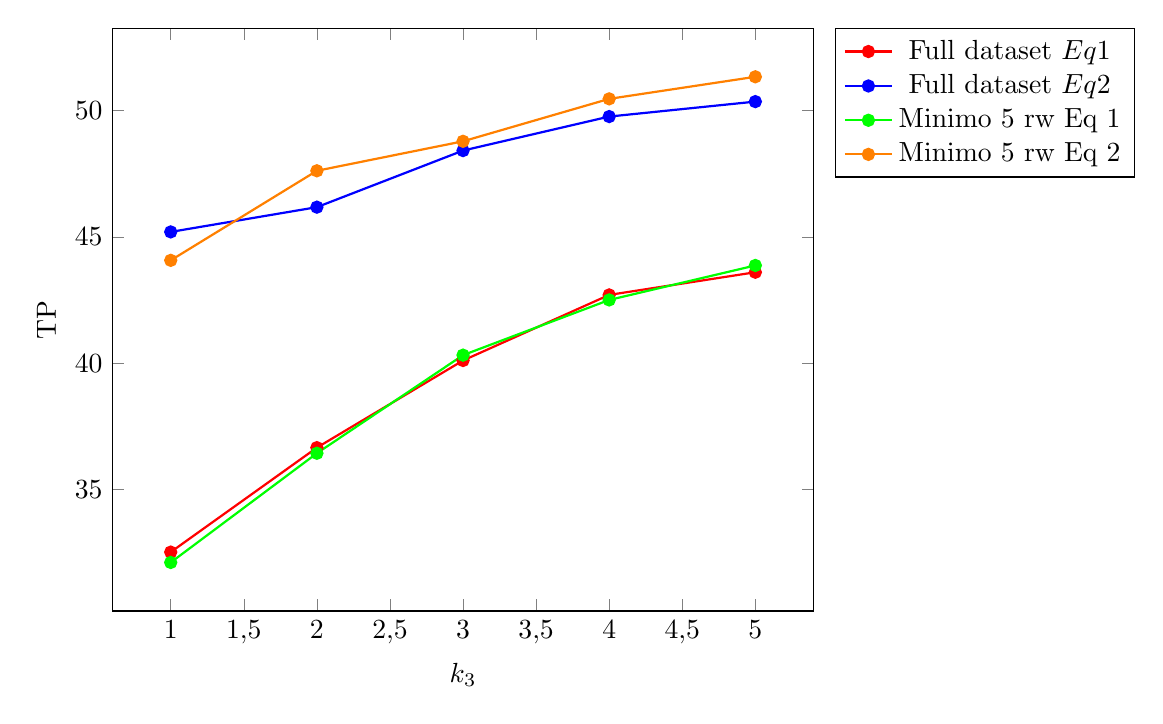
\begin{tikzpicture}
\begin{axis}[scale=1.3,xlabel=$k_3$,ylabel=TP,
%ymode=log,
%scale only axis,
%log origin=infty,
legend pos=outer north east]
% K_3 = 1
%    K_1 = 1
\addplot[thick,mark=*, red] plot coordinates {
(1,32.5139664804)
(2,36.6524129505)
(3,40.1051625239)
(4,42.7038626609)
(5,43.6015006253)	 
}; 
%    K_1 = 2
\addplot[thick,mark=*, blue] plot coordinates { 
	(1, 45.1995685005)
  (2, 46.1801596351)
  (3, 48.4223811527 ) 
  (4, 49.7695852535)
  (5,50.3622047244)
}; 
%    K_1 = 3
\addplot[thick,mark=*, green] plot coordinates {
	(1,32.1029082774)
  (2, 36.4294330519) 
  (3, 40.3173121792)
  (4, 42.5041876047)
  (5, 43.8704387044)
};
%    K_1 = 4
\addplot[thick,mark=*, orange] plot coordinates {
  (1, 44.0732758621)
  (2, 47.6217440544)
  (3, 48.7896494157)
  (4, 50.4712041885)
  (5, 51.3454317897)
}; 

\legend{Full dataset $Eq 1$,Full dataset $Eq 2$,Minimo 5 rw Eq 1,Minimo 5 rw Eq 2}
\end{axis}
\end{tikzpicture}
\label{fig:1}
\caption{TP/Raccomandazioni effettive al variare del numero di raccomandazioni per utente.}
\end{figure}


\subsection{30\% TEST SET}

\begin{figure}[H]
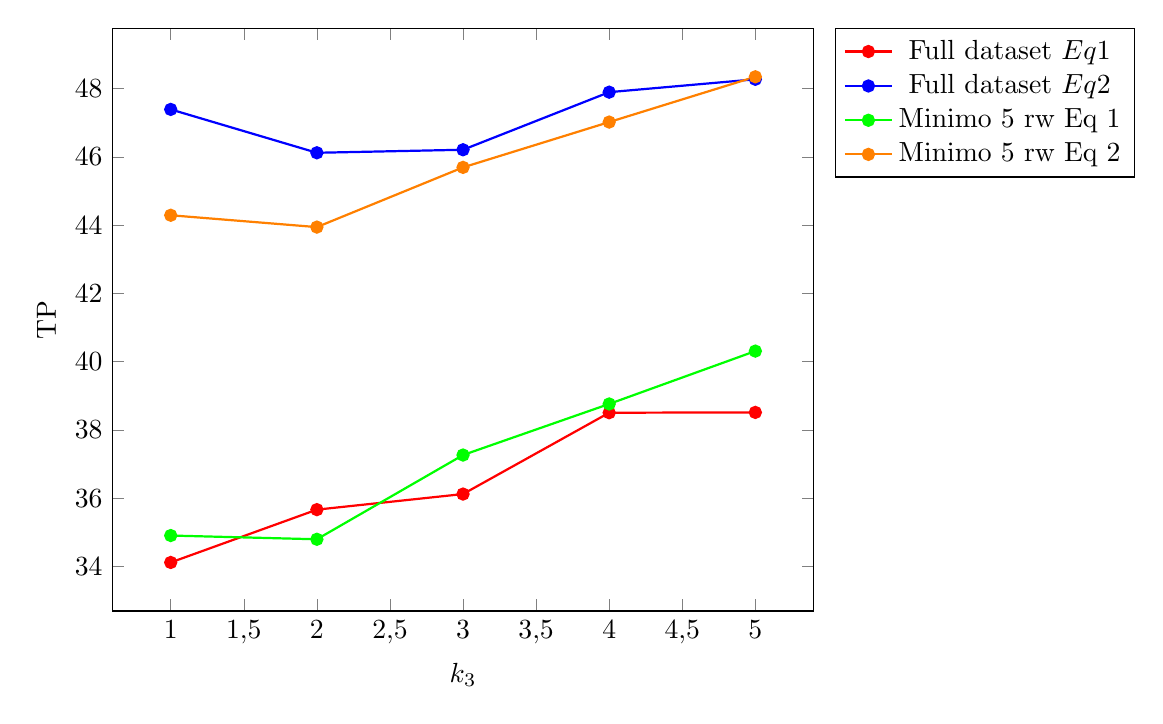
\begin{tikzpicture}
\begin{axis}[scale=1.3,xlabel=$k_3$,ylabel=TP,
%ymode=log,
%scale only axis,
%log origin=infty,
legend pos=outer north east]
% K_3 = 1
%    K_1 = 1
\addplot[thick,mark=*, red] plot coordinates {
(1,34.1201716738)
(2,35.6673960613)
(3,36.123853211)
(4,38.5062748699)
(5,38.5157096425)	 
}; 
%    K_1 = 2
\addplot[thick,mark=*, blue] plot coordinates { 
	(1, 47.3908413206)
  (2, 46.1204557786)
  (3, 46.2089777442) 
  (4, 47.8961504029)
  (5,48.2731757985)
}; 
%    K_1 = 3
\addplot[thick,mark=*, green] plot coordinates {
  (1,34.9087003222)
  (2, 34.7993402969) 
  (3, 37.2668443091)
  (4, 38.7630128598)
  (5, 40.3115605357)
};
%    K_1 = 4
\addplot[thick,mark=*, orange] plot coordinates {
  (1, 44.2902881537)
  (2, 43.9435089625)
  (3, 45.6928838951)
  (4, 47.020065888)
  (5, 48.3464566929)
}; 

\legend{Full dataset $Eq 1$,Full dataset $Eq 2$,Minimo 5 rw Eq 1,Minimo 5 rw Eq 2}
\end{axis}
\end{tikzpicture}
\label{fig:2}
\caption{TP/Raccomandazioni effettive al variare del numero di raccomandazioni per utente.}
\end{figure}




\end{document}
